%%%%%%%%%%%%%%%%%%%%%%%%%%%%%%%%%%%%%%%%%
% Thin Sectioned Essay
% LaTeX Template
% Version 1.0 (3/8/13)
%
% This template has been downloaded from:
% http://www.LaTeXTemplates.com
%
% Original Author:
% Nicolas Diaz (nsdiaz@uc.cl) with extensive modifications by:
% Vel (vel@latextemplates.com)
%
% License:
% CC BY-NC-SA 3.0 (http://creativecommons.org/licenses/by-nc-sa/3.0/)
%
%%%%%%%%%%%%%%%%%%%%%%%%%%%%%%%%%%%%%%%%%

%----------------------------------------------------------------------------------------
%	PACKAGES AND OTHER DOCUMENT CONFIGURATIONS
%----------------------------------------------------------------------------------------

\documentclass[a4paper, 11pt]{article} % Font size (can be 10pt, 11pt or 12pt) and paper size (remove a4paper for US letter paper)

\usepackage[utf8]{inputenc}
\usepackage[T1]{fontenc}
\usepackage[francais]{babel}

\usepackage[protrusion=true,expansion=true]{microtype} % Better typography
\usepackage{graphicx} % Required for including pictures
\usepackage{wrapfig} % Allows in-line images

\usepackage{amsmath}

\usepackage{mathpazo} % Use the Palatino font
\linespread{1.05} % Change line spacing here, Palatino benefits from a slight increase by default

\makeatletter
\renewcommand\@biblabel[1]{\textbf{#1.}} % Change the square brackets for each bibliography item from '[1]' to '1.'
\renewcommand{\@listI}{\itemsep=0pt} % Reduce the space between items in the itemize and enumerate environments and the bibliography

\renewcommand{\maketitle}{ % Customize the title - do not edit title and author name here, see the TITLE block below
\begin{flushright} % Right align
{\LARGE\@title} % Increase the font size of the title

\vspace{50pt} % Some vertical space between the title and author name

{\large\@author} % Author name
\\\@date % Date

\vspace{40pt} % Some vertical space between the author block and abstract
\end{flushright}
}

%----------------------------------------------------------------------------------------
%	TITLE
%----------------------------------------------------------------------------------------

\title{\textbf{Synthèse Bibliographique}\\ % Title
Les Systèmes de Notations} % Subtitle

\author{\textsc{Brunisholz, Di Folco, Pigeon} % Author
\\{\textit{INSA Lyon}}} % Institution

\date{\today} % Date

%----------------------------------------------------------------------------------------

\begin{document}

\maketitle % Print the title section

%----------------------------------------------------------------------------------------
%	ABSTRACT AND KEYWORDS
%----------------------------------------------------------------------------------------

%\renewcommand{\abstractname}{Summary} % Uncomment to change the name of the abstract to something else

\begin{abstract}
	Ce document de synthèse a pour but de traiter des systèmes de réputation en informatique.
	Il abordera ainsi les systèmes de réputation dans leur généralité en guise d'introduction.
	Sera ensuite présenté un état de l'art des différents algorithmes de notations.
\end{abstract}

%\hspace*{3,6mm}\textit{Keywords:} lorem , ipsum , dolor , sit amet , lectus % Keywords

\vspace{30pt} % Some vertical space between the abstract and first section

%----------------------------------------------------------------------------------------
%	ESSAY BODY
%----------------------------------------------------------------------------------------

\section{Introduction}
Les systèmes de réputation sont à la base de nos prises de décisions, en l'absence de meilleurs informations concernant celles-ci.
Ils ont de ce fait une part extrement importante depuis l'apparition d'internet, car en l'absence de métriques concernant la qualité d'un contenu Web,
il serait quasiment impossible pour une personne de trouver un résultat pertinant lors d'une recherche internet, d'estimer le risque avant un achat en ligne,
de s'assurer de la qualité d'un contenu consommé, etc...
Ayant conscience de l'enjeu qu'ils représentent, il est donc intéressant de se pencher sur ceux-ci, afin de comprendre leur fonctionnement.

%Ainsi, en guise d'introduction, il sera proposé de voir ce qu'est une réputation, et quelles sont les caractéristiques générales d'un système de réputation.

\section{Aspect des systèmes de réputation}
Cette partie a pour but d'introduire différents termes et concepts concernant les systèmes de réputation en général afin de mieux apréhender le sujet.

\subsection{Généralités}
\subsubsection{Définitions}
Nous allons essayer ici de donner les définitions de deux concepts fondamentaux des systèmes de réputation.

\paragraph{La réputation}
De manière naïve, la réputation pourrait se réduire au fait que quelqu'un apporte un jugement sur quelque chose~\cite{FarmerGlass2010}.
Le jugement apporté, peut quand à lui être de deux types distincts~\cite{FarmerGlass2010}.
\begin{description}
	\item[Explicite] Le jugement émis peut être directe ou indirecte, mais quoi qu'il en soit, il s'agit d'une affirmation émise par l'auteur du jugement.
	\item[Implicite] Le jugement n'est plus une affirmation, mais un comportement. C'est en effet l'action d'une personne vis à vis d'un sujet qui atteste de la réputation de celui-ci.
\end{description}

\paragraph{La confiance}
La confiance est intimement liée à la réputation. Comme dit précédemment, il s'agit d'estimer sa décision avec un montant d'information minimal.
Cette prise de risque repose sur la confiance que l'on attribue à une réputation, dont l'on peut donner les définitions suivantes :
\begin{description}
	\item[Définition 1] Trust is the subjective probability by which an in-dividual, A, expects that another individual, B, performs a given action on which its welfare depends~\cite{JosangIsmailBoyd2007}.
	\item[Définition 2]Trust is the extent to which one party is willing to depend on something or somebody in a given situation with a feeling of relative security, even though negative consequences are possible~\cite{JosangIsmailBoyd2007}.
\end{description}

Cependant, il n'est pas possible de définir formellement la confiance, car un modèle de celle-ci est difficile à établir sans singulariser cette dernière.

\subsubsection{Donner son avis}
Il s'agit ici de donner un aperçu des différents moyen d'exprimer et de restituer un avis.

\paragraph{Métriques discrètes}
Les métriques discrètes sont pour le plus souvent des affirmations verbales qualitative concernant le contenu noté ou à noter.
Elles sont utilisées car il est plus facile pour une personne de raisonner avec ce type de métriques plutôt qu'avec des systèmes continusi~\cite{JosangIsmailBoyd2007}.
Cependant ces métriques ne sont pas facilement manipulable dans les algorithmes de calculs de réputations.
Ils utilisent alors des systèmes d'heuristiques afin de les exploiter.

\paragraph{Métriques continues}
A l'inverse des métriques discrètes, les mériques continues sont facilement exploitable par les algorithmes de calculs de réputations.
Ils sont souvent utilisés dans des systèmes ne nécessitant pas l'intervention humaine afin d'obtenir des informations concernant la qualité d'un contenu.

\subsection{Différentes classes d'algorithmes}
\subsubsection{User driven}
Dans ce type d'algorithmes il est question de demander à l'utilisateur de qualifier la qualité d'un contenu qu'il a consulté~\cite{Tulungan2013}.
Il s'agit le plus souvent d'une réputation explicite.
Beaucoup de sites Web utilisent ce genre de systèmes.

\subsubsection{Content driven}
Dans ces systèmes de réputation, la qualité d'une contribution est évaluée par son contenu~\cite{Tulungan2013}.
Contrairement aux algorithmes user driven, ici l'évaluation se fait à l'insu de l'utilisateur.
Il s'agit le plus souvent d'un calcul de réputation implicite.
On peut par exemple cité le systèmes de réputation de pages de l'encyclopédie Wikipedia (WikiTrust) qui utilise cette approche afin d'évaluer la qualité des articles~\cite{WikiTrustSite}.

\subsubsection{Centralisé}
Les systèmes de réputations peuvent avoir une architecture centralisée~\cite{JosangIsmailBoyd2007}.
Ils reposent alors sur la notion d'autorité centrale.
Il s'agit d'un centre de réputation ayant pour rôle de collecter l'ensemble des évaluations auprès des différents participants, de calculer les différentes réputationsi, et de les rendre publiquement accessible pour l'ensemble des participants.
On a donc deux caractéristiques importantes des systèmes centralisés :
\begin{description}
	\item[Un protocole de communication centralisé]permettant de communiquer avec le centre de réputation, aussi bien pour soumettre une note, que pour consulter les différentes réputations.
	\item[Un système de calcul de réputation centralisé]collectant les votes dans le but d'évaluer l'ensemble des participants.
\end{description}

\subsubsection{Distribué}
Les systèmes de réputation distribués ne possèdent pas d'autorité centrale à laquelle se réferrer et / ou soumettre des votes~\cite{JosangIsmailBoyd2007}.
Par contre ces systèmes possèdent de multiples "entrepots" consultable à la demande.
Il s'agit le plus souvent des différents participants au système qui enregistre l'historique de leur transactions.
Comme pour les sytèmes centralisés, on observe deux caractéristiques fondamentales :
\begin{description}
	\item[Un protocole de communication décentralisé]offrant la possibilité aux différents participants de trouver et de consulter "l'historique" d'un membre avant une transaction.
	\item[Un système de calcul de réputation décentralisé commun]permettant de calculer une métrique de réputation grâce à "l'historique" précedemment récupéré.
\end{description}

\subsection{Une architecture partagée}
Par ailleurs, les systèmes de réputation sont généralement tous fondés autour de trois axes principaux~\cite{HoffmanZageNita2007} : la Formulation, l'Application et la Dispersion.

\subsubsection{La Formulation}
C'est au cours de cette étape que l'algorithme de calcul de réputation est enoncé dans sa formulation théorique.
Plus précisement, c'est au cours de cette phase que sont exprimés comment seront colléctée les données utilisées, ainsi que leurs type.
Enfin, il est précisé sous quelle forme l'algorithme rendra son résultat. Celui-ci peut être binaire, discret ou continu.

\subsubsection{L'Application}
Il s'agit de l'implémentation de l'algorithme.
Contrairement à la Formulation, cette étape prends en compte les différentes contraintes du milieu dans lequel l'algorithme va être appliqué.
Il s'agit alors de respecter la métrique voulue, tout en essayant d'être resistant aux attaques malicieuses.
Ainsi il est notamment discuté des méthodes de stockage et de calculs qui vont être utilisées.

\subsubsection{La Dispersion}
La Dispersion correspond aux méthodes employées afin de transmettre l'information relative à la réputation d'une entité aux différents acteurs concernés.
Il sera alors discuté de la manière dont la réputation est stockée, comment celle-ci est transmise, et sa redondance.

\section{Les attaques / faiblesses connues des systèmes de réputations}
\subsection{Définition de la notion d'attaque}
Nous qualifierons d'attaque tout usage détourné du système de réputation,
c'est-à-dire, tout ce qui vise à déstabiliser le système pour qu'il y ait une
perte de confiance des acteurs réels en celui-ci due à une réputation calculée
différente de la réputation réelle.

Les acteurs réels sont tous les acteurs qui utilisent le système de réputation
comme base pour leur décisions.

\subsection{Les grandes familles de comportement malicieux}
\subsubsection{L'auto promotion}
L'auto-promotion est un procédé qui vise à augmenter artificiellement la réputation
d'un acteur.

L'approche classique pour atteindre cet objectif consiste à créer un grand nombre
de comptes (ou à simuler un grand nombre d'acteurs anonyme quand le système le permet)
et à émettre un grand nombre d'avis positifs à destiné de l'acteur que l'on souhaite
promouvoir.

Cette technique est également utilisée pour la discréditation artificielle.

\subsubsection{L'usurpation d'identité}
L'usurpation d'identité est une attaque qui vise le système d'authentification,
elle à pour but de prendre l'identité d'un acteur donné pour lui faire faire des
actions précise dans le but d'altérer artificiellement sa propre réputation ou celle
d'un autre.

\subsubsection{Wormhole / Blackhole}

\section{Présentation des algorithmes et de leurs approches mathématiques}
\subsection{Captcha}
\subsubsection{Concept}
Les captcha sont des tests de tests de Turing ayant pour but de différencier une machine d'un humain.
Il s'agit le plus souvent d'une image représentant un mot déformé visuellement rendant ainsi les algorithmes de reconnaissance de caractères difficilement utilisables.
Il peut aussi s'agir de reconnaissance de son, chose tout aussi difficile à traiter algorithmiquement.
Il est alors demandé à l'utilisateur d'entrer la valeur de ce qu'il lui a été demandé de reconnaitre, afin de prouver qu'il est bien un humain.

Nous allons voir un algorithme de calcul de réputation reposant sur le concept de captcha.

\subsubsection{Tulungan}
Il s'agit d'un algorithme colaboratif (user-driven) permettant de donner une métrique sur le contenu d'une URL, en lui associant une ou plusieurs catégories d'URLs.
L'algorithme part du postulat qu'un utilisateur peut à la fois contribuer à la classification de contenu, et noter du contenu.
Il s'éxécute en trois phase : la phase d'Initialisation, la phase de Contribution et Notation, et la phase de Calcul~\cite{Tulungan2013}.

La phase d'Initialisation a lieu à chaque fois qu'un nouvel uilisateur apparaît, ou qu'une nouvelle catégorie d'URL est crée.
Ainsi les valeurs de contributions et de notations sont initialisées avec une valeur proche de zéro.

La phase de contribution et de notation permet à chaque participants de prendre part à la catégorisation en exprimant si un contenu web appartient ou non à différentes catégories.
Par ailleurs au cours de cette phase seront choisit des noteurs potentiels (car ils sont susceptibles de donner une mauvaise métrique) en fonction de leurs précédentes contributions et notations.
Ceci a pour but de séléctionner des personnes en rapport avec le contenu qu'il leurs sera demandé de noter.
Dernière étape de cette phase, la notation à proprement parler. Les participants doivent alors noter trois URLs en exprimant si elles sont bien catégorisées.
Deux des URLs sont des URLs de contrôle, dont les catégories d'appartenances sont bien connues.
La dernière est quand à elle l'URL dont on souhaite déterminer si la catégorisation est pertinente ou non.
Les trois URLs sont présentées de manière à ce que l'utilisateur ne sache pas laquelle est la réelle cible de l'algorithme.
L'algorithme considère alors que si un utilisateur réponds correctement aux deux URLs connu, alors il est probable que celui-ci ai répondu de manière sérieuse à la troisième.
Cette approche peut être comparée aux Captcha.

La dernière phase de l'algorithme consiste à reévaluer l'ensemble des réputations des URLs, des noteurs et des contributeurs.

\subsubsection{Forces}
Tulungan est un algorithme dit "consensu-independant", car il n'a besoins que de 20\% de participants honnêtes pour être efficace, là où des algorithmes plus classiques necessitent une proportion de participants honnêtes de l'ordre de 50\%.
Ce traits lui permet ainsi de résister à l'auto-promotion (modélisé dans l'article par une attaque Sybile)~\cite{Tulungan2013}.

\subsubsection{Faiblesses}
Tulungan est relativement couteux en "main d'oeuvre humaine" ce qui peut être problématique dans certains cas, et qui interdit de l'utiliser dans un contexte entièrement automatisé.
Par ailleurs nous ne savons actuellement pas comment réagit ce système à d'autres types d'attaques.

\subsection{Loi de Beta}
\subsubsection{Concept}
L'idée fondatrice de la Loi de Beta détaillée dans %% TODO ref Loi de Beta
est que les actions du passées sont condamnées à se reproduire.

L'approche consiste donc à évaluer à postériori les actions qui ont eu lieu
afin de déterminer une réputation représentant les actions futures.

\subsubsection{Algorithme}
L'algorithme comporte une partie qui calcul la réputation des utilisateurs à partir d'un ensemble d'entrées (comme les notes d'eBay).
Le point centrale est la fonction de densité Beta qui est utilisée pour représenter la probabilité d'événements binaires (feedback positif ou négatif).
Ensuite, la fonction de réputation se repose sur la fonction Beta, mais au lieu de fournir une entrée binaire (un couple de nombre de feedback positif et négatif), fournis un couple de degrés de réputation.
Une fonction d'évaluation de la réputation obtenue qui permet de convertire un résultat mathématique en résultat humainement interprêtable via une conversion en probabilité.
La récolte des données est un point important, car afin d'établir une réputation de nombreuses sources sont exploitées et de nombreux feedbacks sont récoltés provenant de différent agents. Ces agents n'ont pas tous la même réputation, ainsi, les feedbacks sont pondérés en fonction de la réputation de ceux qui les émettent.
Ces données sont à filtrer en fonction de leur ancienneté, en effet, un agent peut changer de comportement au cours du temps, le modèle inclura donc un facteur d'oublie pour résoudre ce problème.

Enfin, une seconde partie qui vise à stocker et à accéder aux réputations (centralisée comme chez eBay ou décentralisée comme dans PGP).

\subsubsection{Forces}
Il s'agit d'un système simple et suffisemment flexible pour s'adapter à un grand nombre de situations, il permet de résister à l'auto-promotion, à la discréditation artificielle ainsi qu'aux changements de comportements et il permet de supporté à la fois une architecture centralisée et décentralisée.

\subsubsection{Faiblesses}
En revanche, cet algorithme met beaucoup de contraintes sur les données entrantes et il présuppose que l'authenfication est en place et est robuste, ce qui ne le prémunis pas, le cas contraire des attaques de la part de multiples comptes ou d'anonymes.

\subsection{2-Phase Machine Learning}
\subsubsection{Concept}
Ce type d'algorithme agit en deux temps.
Comme les documents à évaluer sont souvent complexe, il s'agit dans la première phase, de récupérer un ensemble de métriques sensées caractériser le contenu à évaluer.
Dans le cas de WikiTrust, algorithme que nous allons pas la suite détailler, il s'agit d'une quinzaine d'attributs, dont :
\begin{itemize}
	\item La réputation de l'auteur
	\item L'anonimat de l'auteur
	\item Le temps entre les révisions du contenu
\end{itemize}
Viens ensuite la deuxième phase de l'algorithme, où sont utilisés les métriques précédement calculées afin de calculer l'indice de réputation.
Dans le cas de WikiTrust, il s'agit d'un arbre de décision entrainés au préalable sur des jeux de tests.

Nous allons maintenant présenté WikiTrust dans un cadre plus général.

\subsubsection{WikiTrust}
Il s'agit de l'algorithme utilisé par Wikipedia pour évaluer la réputation des auteurs et des articles. Il repose sur l'analyse des modifications de contenu d'un article.
En effet, si une personne modifie un article sur l'encyclopédie, la réputation de l'article varie de la manière suivante~\cite{WikiTrust2010}~\cite{WikiTrustSite} :
ce qui a été réécrit gagne un petit montant de réputation pondéré par la réputation de l'auteur,
et la partie restée inchangée gagne elle aussi en réputation en fonction de la réputation du modificateur, et de son temps restée inchangée.
L'indice de confiance global de l'article est ensuite réévalué.

La réputation d'un auteur est calculée d'une manière similaire, à savoir que lorsqu'un article est modifié,
la réputation de l'auteur original est elle aussi modifié en fonction de la quantité de contenu modifié, pondérée par la réputation du modificateur.

\subsubsection{Forces}
WikiTrust part du postulat que les personnes malveillante possède pas ou peu de réputations, ce qui rends l'algorithme de calcul de réputation resistant à l'auto promotion~\cite{Tulungan2013}.

\subsubsection{Faiblesses}
Partant du même postulat, une personne possédant une haute réputation, et décidant de devenir malveillante à postériori, peu alors corrompre le système.

\subsection{Network flow}
\subsubsection{Concept}
Les algorithmes de type Network Flow sont une application de la théorie des graphes.
Il s'agit de donner à un noeud (supposé extrèmement fiable) une valeur de départ appelée "énergie", qui dans le cadre des systèmes de réputations, correspond à une valeur de confiance distribuable~\cite{ZieglerLausen2005}.
Viens ensuite l'étape au cours de laquelle le noeud de départ va devoir "énergiser" les noeuds avec lesquels il a eu un contact (au sens transaction nécessitant une confiance), à hauteur de la qualité de l'échange.
Cependant, le noeud ne peut distribuer qu'un nombre finit d'"énergies" correspondant à la valeur de son énergie de départ.
Il devra donc diviser celle-ci afin de la distribuer pour l'ensemble des noeuds, chaque noeud recevant un montant pondéré par la qualité de la transaction.

Les noeuds ayant reçu de l'"énergie" peuvent à leur tour distribuer celle-ci aux noeuds avec lesquels ils effectuent des transactions en suivant les règles définies précédement.

Enfin ce système de réputation possède un nombre de valeurs de réputation distribuable sont souvent fini.

\subsubsection{EigenTrust}
EigenTrust est un algorithme basé sur une structure Network flow. Il est utilisé dans les réseaux Peer to Peer afin d'évaluer les participants du réseau~\cite{KamvarSchlosserGarciaMolina2003}.
Il fonctionne en plusieurs étapes.

\paragraph{Normalisation de la confiance locale}
Afin d'éviter qu'un participant malicieu puisse donner des valeurs de confiances arbitrairement élevée à d'autres participants malicieux, et au contraire des valeurs de confiance basse aux participants honnêtes, l'algorithme commence par effectuer une normalisation de la confiance locale selon la formule suivante :
\begin{center}
	$c_{ij} = \frac{\max{(s_{ij},0)}}{\sum \max{(s_{ij},0)}}$
\end{center}
Avec $s_{ij} = \sum tr_{ij}$ et $tr_{ij}$ correspondant à la qualité d'une transaction entre un participant $i$ et un participant $j$, et pouvant prendre pour valeur $1$ ou $-1$.
\paragraph{}
Cette normalisation permet alors de ramener la confiance locale entre $0$ et $1$.
Par ailleurs elle permet de pouvoir comparer les confiances d'un noeud par rapports aux différents noeuds qu'il a noté, sans pour autant savoir s'il s'agit de bonnes ou de mauvaises réputations.

\paragraph{Aggrégation des valeurs de confiances locale}
Viens ensuite une étape d'aggrégation des différentes valeurs de confiances locales pour chaque noeud.
Supposons qu'un noeud $i$ souhaite aggreger les différentes valeurs de confiances locale d'un noeud $k$, il va alors demander à tous les noeuds qu'il connait la confiance que ceux-ci donnent au noeud $k$, et ponderera cette confiance par la confiance qu'il accorde aux noeuds intérogés.
On a donc la relation suivante :
\begin{center}
	$t_{ik} = \sum_{j} c_{ij}c_{jk}$
\end{center}
Si cette étape est étendu à une echelle globale, à savoir si un noeud demande à ses noeuds voisins qui eux même demandent à leurs noeuds voisins, et ainsi de suite, $t$ converge alors vers la valeur de confiance que l'ensemble des participants a envers un noeud.

\subsubsection{Forces}
Ce type d'approche permet de réduire considérablement le nombre de noeuds malicieux "solitaires", et grâce à la normalisation et à l'aggrégation, l'auto-promotion est fortement atténuée.

\subsubsection{Faiblesses}
Le système est cependant faiblement résistant à la notion de consensus.
En effet, il suffirait d'un nombre de noeuds malicieux appartenant à un même groupe, et représentant 40\% des participants au système afin d'influencer le système de réputation.
Dans la pratique, il est quasiment impossible d'obtenir une telle proportion de noeuds malicieux dans un réseau Peer to Peer.

\subsection{MANET (Trouver le vrai nom)}

\section{Conclusion}
\subsection{Matrice de comparaison}
\subsection{Questions ouvertes}

\section{Etat de l'art}
Il s'agit dans cette partie de voir quels sont les différents systèmes de réputations actuels, et de les comparer.


\subsection{Karma}
\subsubsection{Concept}
Le Karma permet d'évaluer la réputation uniquement d'une personne au sein d'une communauté Web. Le nombre de points Karma est attribué en fonction :
\begin{itemize}
	\item De la vieillesse de l'utilisateur au sein de la communauté
	\item Des actions auxquelles il a participé
	\item Des résultats qu'il a obtenus
	\item De ce que pense les autres utilisateurs
\end{itemize}
Inclure le Karma dans le système de réputation d'un site Web permet de rendre celui-ci plus performant et plus proche de la réalité. Il est d'ailleurs rarement utilisé seul pour cacluler une réputation mais associé à d'autres algorithmes.

Il existe deux formes de Karma et une combinaison :
\begin{description}
	\item[Participation] calcule le Karma en fonction de la participation du membre de a communauté
	\item[Qualité] calcule le Karma en fonction de la qualité des contributions du membre
	\item[Robuste] est une combinaison des deux précédentes
\end{description}

\subsubsection{Calcul du Karma, modèle de participation}
La calcul de la réputation grâce à ce modèle se fait via l'attribution de points. Lorsqu'un membre effectue une action au sein de la communauté, un nombre de points lui est attribué en fonction de cette action. La réputation de ce membre est donc la somme des points obtenus.

Il existe également, un système de points négatifs. Lorsqu'un membre effectue une mauvaise action, on lui attribue un nombre de points négatifs correspondant à cette mauvaise action. Le système est le même que celui des points positifs, excepté qu'un score élevé correspond à une mauvaise réputation.

\subsubsection{Calcul du Karma, modèle de qualité}
Dans ce modèle, le nombre de contributions n'a pas d'importance. Seule compte la qualité de ces dernières. 

Le modèle de Feedback utilisé par eBay décrit précédemment est un exemple de modèle de qualité du Karma.

\begin{figure}
	\begin{center}
		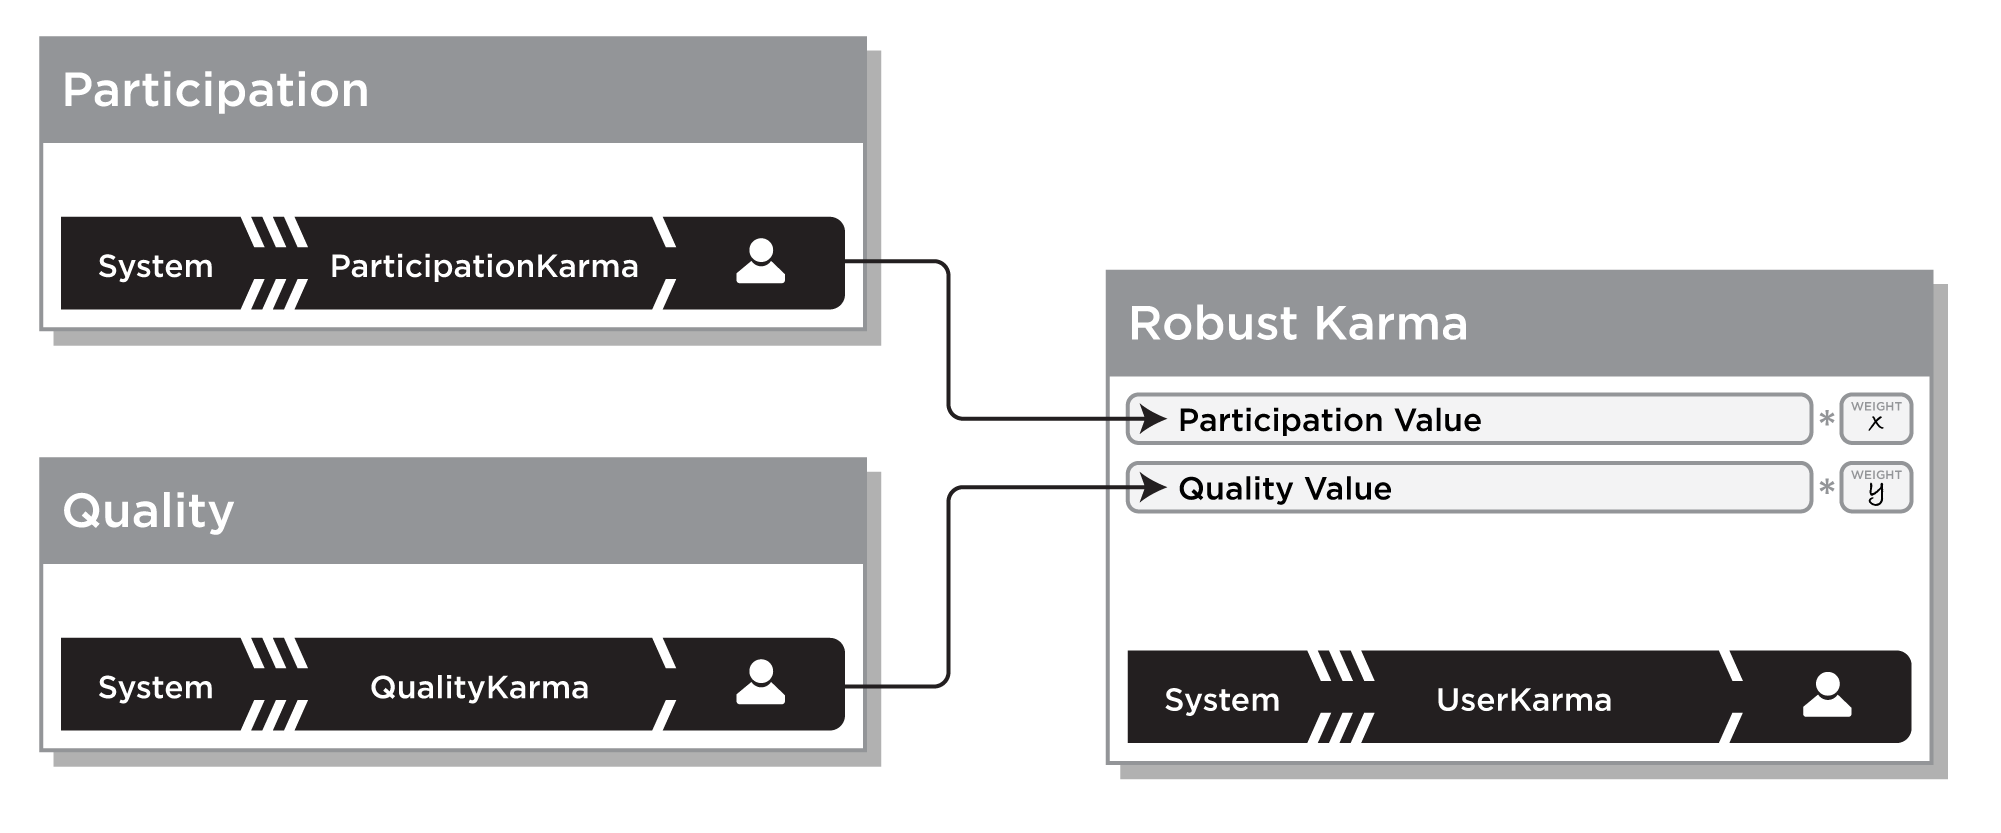
\includegraphics[width=12cm]{karma.png} 
	\end{center}
	\caption{Modèle robuste~\cite{FarmerGlass2010}}
	\label{robusteKarma}
\end{figure}

\subsubsection{Calcul du Karma, modèle robuste}
En combinant les deux modèles précédents, on obtient le modèle robuste, comme le montre la figure~\ref{robusteKarma}. 

\subsubsection{Reddit.com}
Reddit.com est un site communautaire qui permet à chaque membre de soumettre des liens aux autres membres qui peuvent ensuite voter pour ce lien. Les membres peuvent également commenter les liens proposer et voter pour ou contre les commentaires.

A chaque membre est associé un "Karma". Ce dernier est calculé en fonction des votes des membres. Lorsqu'un membre vote pour un lien proposé, le karma du membre qui a proposé le lien est augmenté d'un point. Lorsqu'un membre vote contre un lien proposé, le karma du membre qui a proposé le lien est diminué d'un point. Si le membre a obtenu plus de votes négatifs que de votes positifs, son karma est donc négatif. Les liens proposés par des membres qui ont un bon karma sont plus facilement visibles par les autres membres, que les liens proposés par des membres qui ont un moins bon karma~\cite{RedditTroll}.

De même, le karma d'un membre est augmenté d'un point lorsqu'un autre membre vote pour un de ses commentaires et est diminué d'un point lorsqu'un autre membre vote contre~\cite{RedditTroll}.

\subsubsection{Comment contrôler le karma ?}
Expliquer comment reddit tente de contrer les trolls ?


\subsection{Système de Digg}
\subsubsection{Concept}
Digg est un site web de partage d'article communautaire, un membre lit un article sur internet ou écrit un article sur un espace personnel, puis il le soumet à Digg.
Ensuite les autres membres du site votent pour ou contre cet article et s'il obtient assez de voix il est publié en page d'accueil de Digg.

\subsubsection{Algorithme}
L'algorithme est donc simple : il n'y a pas de votes négatif, la réputation d'un article ne peut que croître, une fois le nombre de voix critique atteint, il est publié en première page, si non, au bout d'un certain temps, l'article est supprimé des propositions.

\subsubsection{Forces}
L'un des principaux avantages est que ce système ne permet pas de discréditation et qu'il n'attise pas l'augmentation artificielle car l'enjeu est moindre, il s'agit d'une question de temps.

\subsubsection{Faiblesses}
En revanche il ne permet pas de réprésentation explicite du désaccord des lecteurs, pour cela il faudrait opposer le nombre de lecteurs et le nombre de votants.

\subsection{Rater-Rating}
\subsubsection{Concept}
Le rater-rating est un système de réputation utilisé pour les sites web collaboratifs. Ce système tente d'encourager les membres à noter.

Les sites collaboratifs ont besoin que des auteurs contrôlent le travail d'autres auteurs afin de s'assurer de la bonne réalisation de celui-ci. Cependant, on ne peut pas être sûr que ce contrôle sera bien effectué. Le but de cette méthode est donc de détecter les auteurs qui ne notent pas correctement ou qui ne notent jamais~\cite{RaterRating}.

Les auteurs choisis pour contrôler le travail d'un autre auteur l'ont été en fonction de leur domaine d'expertise. Malgré cela, les contrôleurs peuvent ne pas noter le travail de la bonne façon.

Grâce à cette méthode, la réputation d'un auteur est calculée en fonction de la qualité de son travail et également en fonction de la qualité de ces notations. Un auteur qui ne note jamais ou presque jamais obtiendra une mauvaise note de notation et sa réputation sera donc diminuée. C'est en cela que ce système permet d'inciter les auteurs à noter~\cite{RaterRating}.

Une des limites de ce système de réputation est qu'un bon noteur peut obtenir une mauvaise réputation si tous les autres noteurs sont des mauvais noteurs avec une bonne réputation. Il faut donc que plus de 50\% des contributeurs soient des personnes honnêtes.

Ce système a pour but de :
\begin{itemize}
	\item inciter les contributeurs à noter
	\item encourager les auteurs à publier
	\item pénaliser les mauvais noteurs
	\item noter le travail afin de lui attribuer une note de crédibilité
	\item noter les notes afin d'attribuer aux notes une note de crédibilité~\cite{RaterRating}
\end{itemize}

\subsubsection{Algorithme}
Cette méthode est notamment utilisée pour noter les contributions sur le site Wikipédia. Son algorithme se décompose de la façon suivante :
\begin{description}
	\item[Déterminer l'ensemble des auteurs noteurs] Cette étape a pour but de déterminer si un auteur \textit{i} a la capacité nécessaire pour noter un travail d'un document \textit{d}. Pour cela, il teste si les références utilisées par l'auteur \textit{i} sont les mêmes que celles utilisées pour réaliser le document \textit{d}. De plus, la proportion des documents référencés dans le travail de l'auteur \textit{i} par rapport aux documents référencés dans le document \textit{d} doit être suffisamment grande. Enfin, et cela paraît évident, l'auteur \textit{i} ne doit pas être un des auteurs du document \textit{d}.
	\item[Obtenir l'ensemble des notes] Chaque auteur précédemment sélectionné peut attribuer au travail \textit{t} une note comprise entre -1 et +1.
	\item[Calculer la note globale] La note du travail \textit{t} est la moyenne des notes données par chaque auteur précédemment sélectionné et pondéré par la réputation de l'auteur. Les notes des auteurs ayant une réputation négative ne sont pas prises en compte. Il est possible qu'aucun des auteurs sélectionnés n'ait donné une note ou qu'il n'existe pas d'auteurs avec une réputation positive pour donner de notes, dans ce cas, une note epsilon est attribuée au travail.
	\item[Calculer la crédibilité de la note] La crédibilité est la moyenne des réputations des auteurs ayant noté le travail et ayant eux-mêmes une réputation positive multipliée par la proportion totale de noteurs ( 1 - 1/nombre de noteurs avec une réputation positive ). Cette multiplication permet d'éviter que l'on attribue une forte crédibilité à une note calculée à partir de peu de noteurs. Si la note vaut epsilon, alors sa crédibilité vaudra également epsilon.

Nous pouvons alors remarquer que la réputation de l'auteur \textit{i} influence non seulement la note d'un travail que celui va évaluer, mais également, la crédibilité de la note globale attribuée.

	\item[Calculer la réputation du contributeur] La réputation du contributeur est la réputation d'un auteur \textit{i} basée sur les notes obtenues pour ses contributions. Si c'est la première contribution de l'auteur, sa réputation de contributeur vaut 0.
\end{description}

%------------------------------------------------

\bibliographystyle{plain}
\bibliography{biblio}

\end{document}
